\documentclass[12pt,a4paper]{report}
\usepackage[polish]{babel}                      % Język polski
\usepackage[utf8]{inputenc}                     % Kodowanie dokumentu
\usepackage[T1]{fontenc}                        % Kodowanie fontów
%\usepackage{lmodern}
\usepackage{times}
\usepackage[cm]{fullpage}                       % Cała strona
\usepackage[pdftex,bookmarks,colorlinks]{hyperref} % Linki w dokumencie PDF
\usepackage{indentfirst}                        % Wcięcia akapitów
\usepackage{graphicx}                           % Grafika w png, jpeg, gif
\pagestyle{headings}
%\graphicspath{{png}}                            % Szuka grafik w katalogu png
\frenchspacing                                  % Kontynentalne odstępy międzyzdaniowe

\title{ConvML 1.2}
\author{Marcin Kacprzak \and Piotr Kulinowski}
\date{$Date$}

\begin{document}

\maketitle
\tableofcontents

\section{Wstęp}
Potrzeba opracowania modelu strukturalnego przenośnika taśmowego wynikła z
informatycznej potrzeby i konieczności wprowadzenia procedury zapisu pełnej
informacji o urządzeniu, która jednoznacznie i spójnie opisywałaby parametry
techniczno-ruchowe i konfigurację przenośnika taśmowego.  Ze względu na
uniwersalność zapisu i chęć popularyzacji modelu strukturalnego wprowadzono
anglojęzyczne nazewnictwo poszczególnych podzespołów.

\begin{figure}
\centering
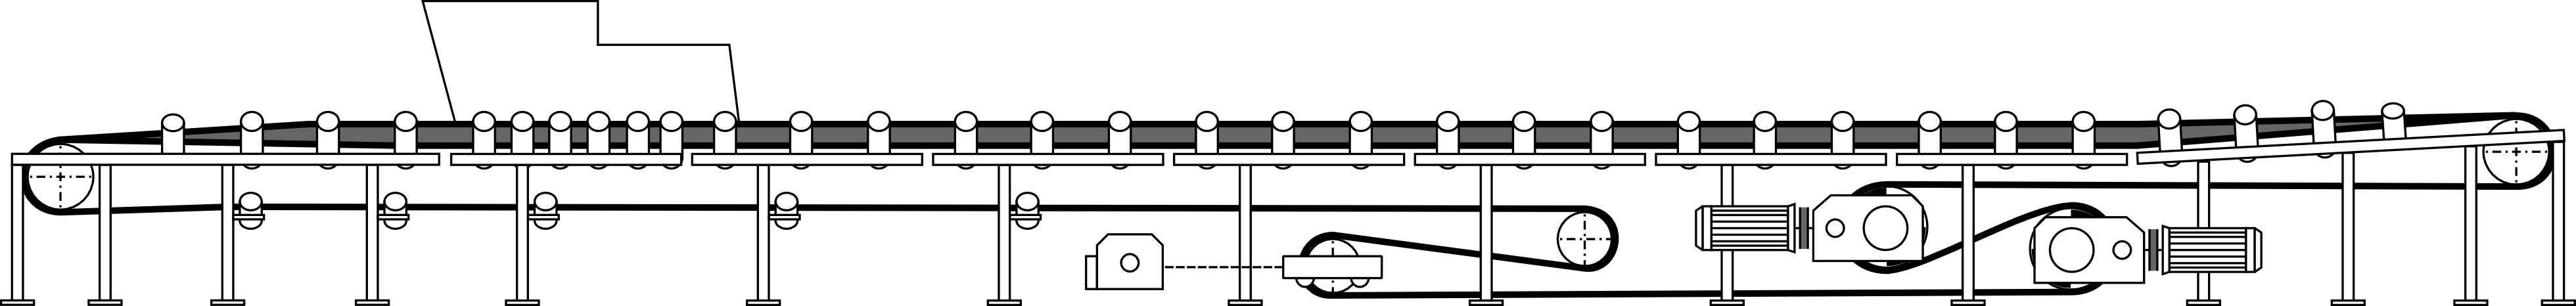
\includegraphics[width=\textwidth]{png/przenosnik}
\caption{Podstawowe podzespoły przenosnika taśmowego}
\label{fig:przenosnik}
\end{figure}

Do opracowania systemu zapisu modelu strukturalnego przenośnika taśmowego
wykorzystano język XML Schema [?89], ułatwiający definiowanie struktury i
kolejności podzespołów przenośnika taśmowego (Tabela 4 1) oraz umożliwiający w
łatwy sposób jego adaptację na platformie informatycznej.  Istotną cechą modelu
strukturalnego jest praktycznie nieograniczona możliwość jego rozbudowy, bez
utraty przejrzystości struktury.  Każdy z elementów posiada grupę atrybutów
opisujących jego cechy, mogące być zarówno parametrami technicznymi jak i
ekonomicznymi.


\end{document}
